The following chapter describes our understanding of Valcon as a company. This includes the environment in which they operate, an analysis of their business model, their business and IT strategies, and an identification of which work domains that affect the problem.

We conducted the analysis before realising that OMT was a big part of the problem, and therefore the analysis in regards to OMT is very limited.

\section{Business environment}
As we are working with internal support functions, we provide only summaries of our environment analyses here.
\subsection{Valcon's environment}
Valcon operates within an competitive environment where image and contacts are key. 
There's a great need for experienced and knowledgeable consultants but there's also a lot of competition in the field.
Not because there are a lot of competitors within the fields that Valcon works in, but rather because the competitors are the same every time.
This means they know each other and know exactly what kind of prices and quality the opposing firms will bring.
Due to this, Valcon's business strategy has been to hire the best and brightest employees and accept the fact that they're unable to be the cheapest organisation to hire.

They sell themselves mainly on knowledge and quality, rather than on price and pride themselves on being a company capable of the entire consultation process, from analysis to implementation.

They refer to themselves as the 'how' company, as they are often employed in projects where a competing consultation firm has been hired to write the analysis report and figure out 'what' to do. 
Valcon are then employed to conclude the project by implementing the solution.

Valcon's biggest threat is losing their consultants.
Consultants are drawn towards new and exciting opportunities, while working for the same company for a long time gets increasingly stale.
This means that sooner or later a consultant will grow tired of the current challenges he's facing and move on to another company. \todo{SOURCES}
\subsection{OMT's environment}
OMT primarily works with warships, a field they're not facing a lot of competition within. 
This also enables them to subcontract other companies, since they're not direct competition and therefore don't mind.
A more thorough investigation of OMT's environment can be found in appendix \ref{app:OMT_environment}.
\section{Valcon's business model}
The business canvas gives an overview of Valcon's business.
Based on our analysis we have the following understanding of Valcon's canvas.
\begin{figure}[!htp]
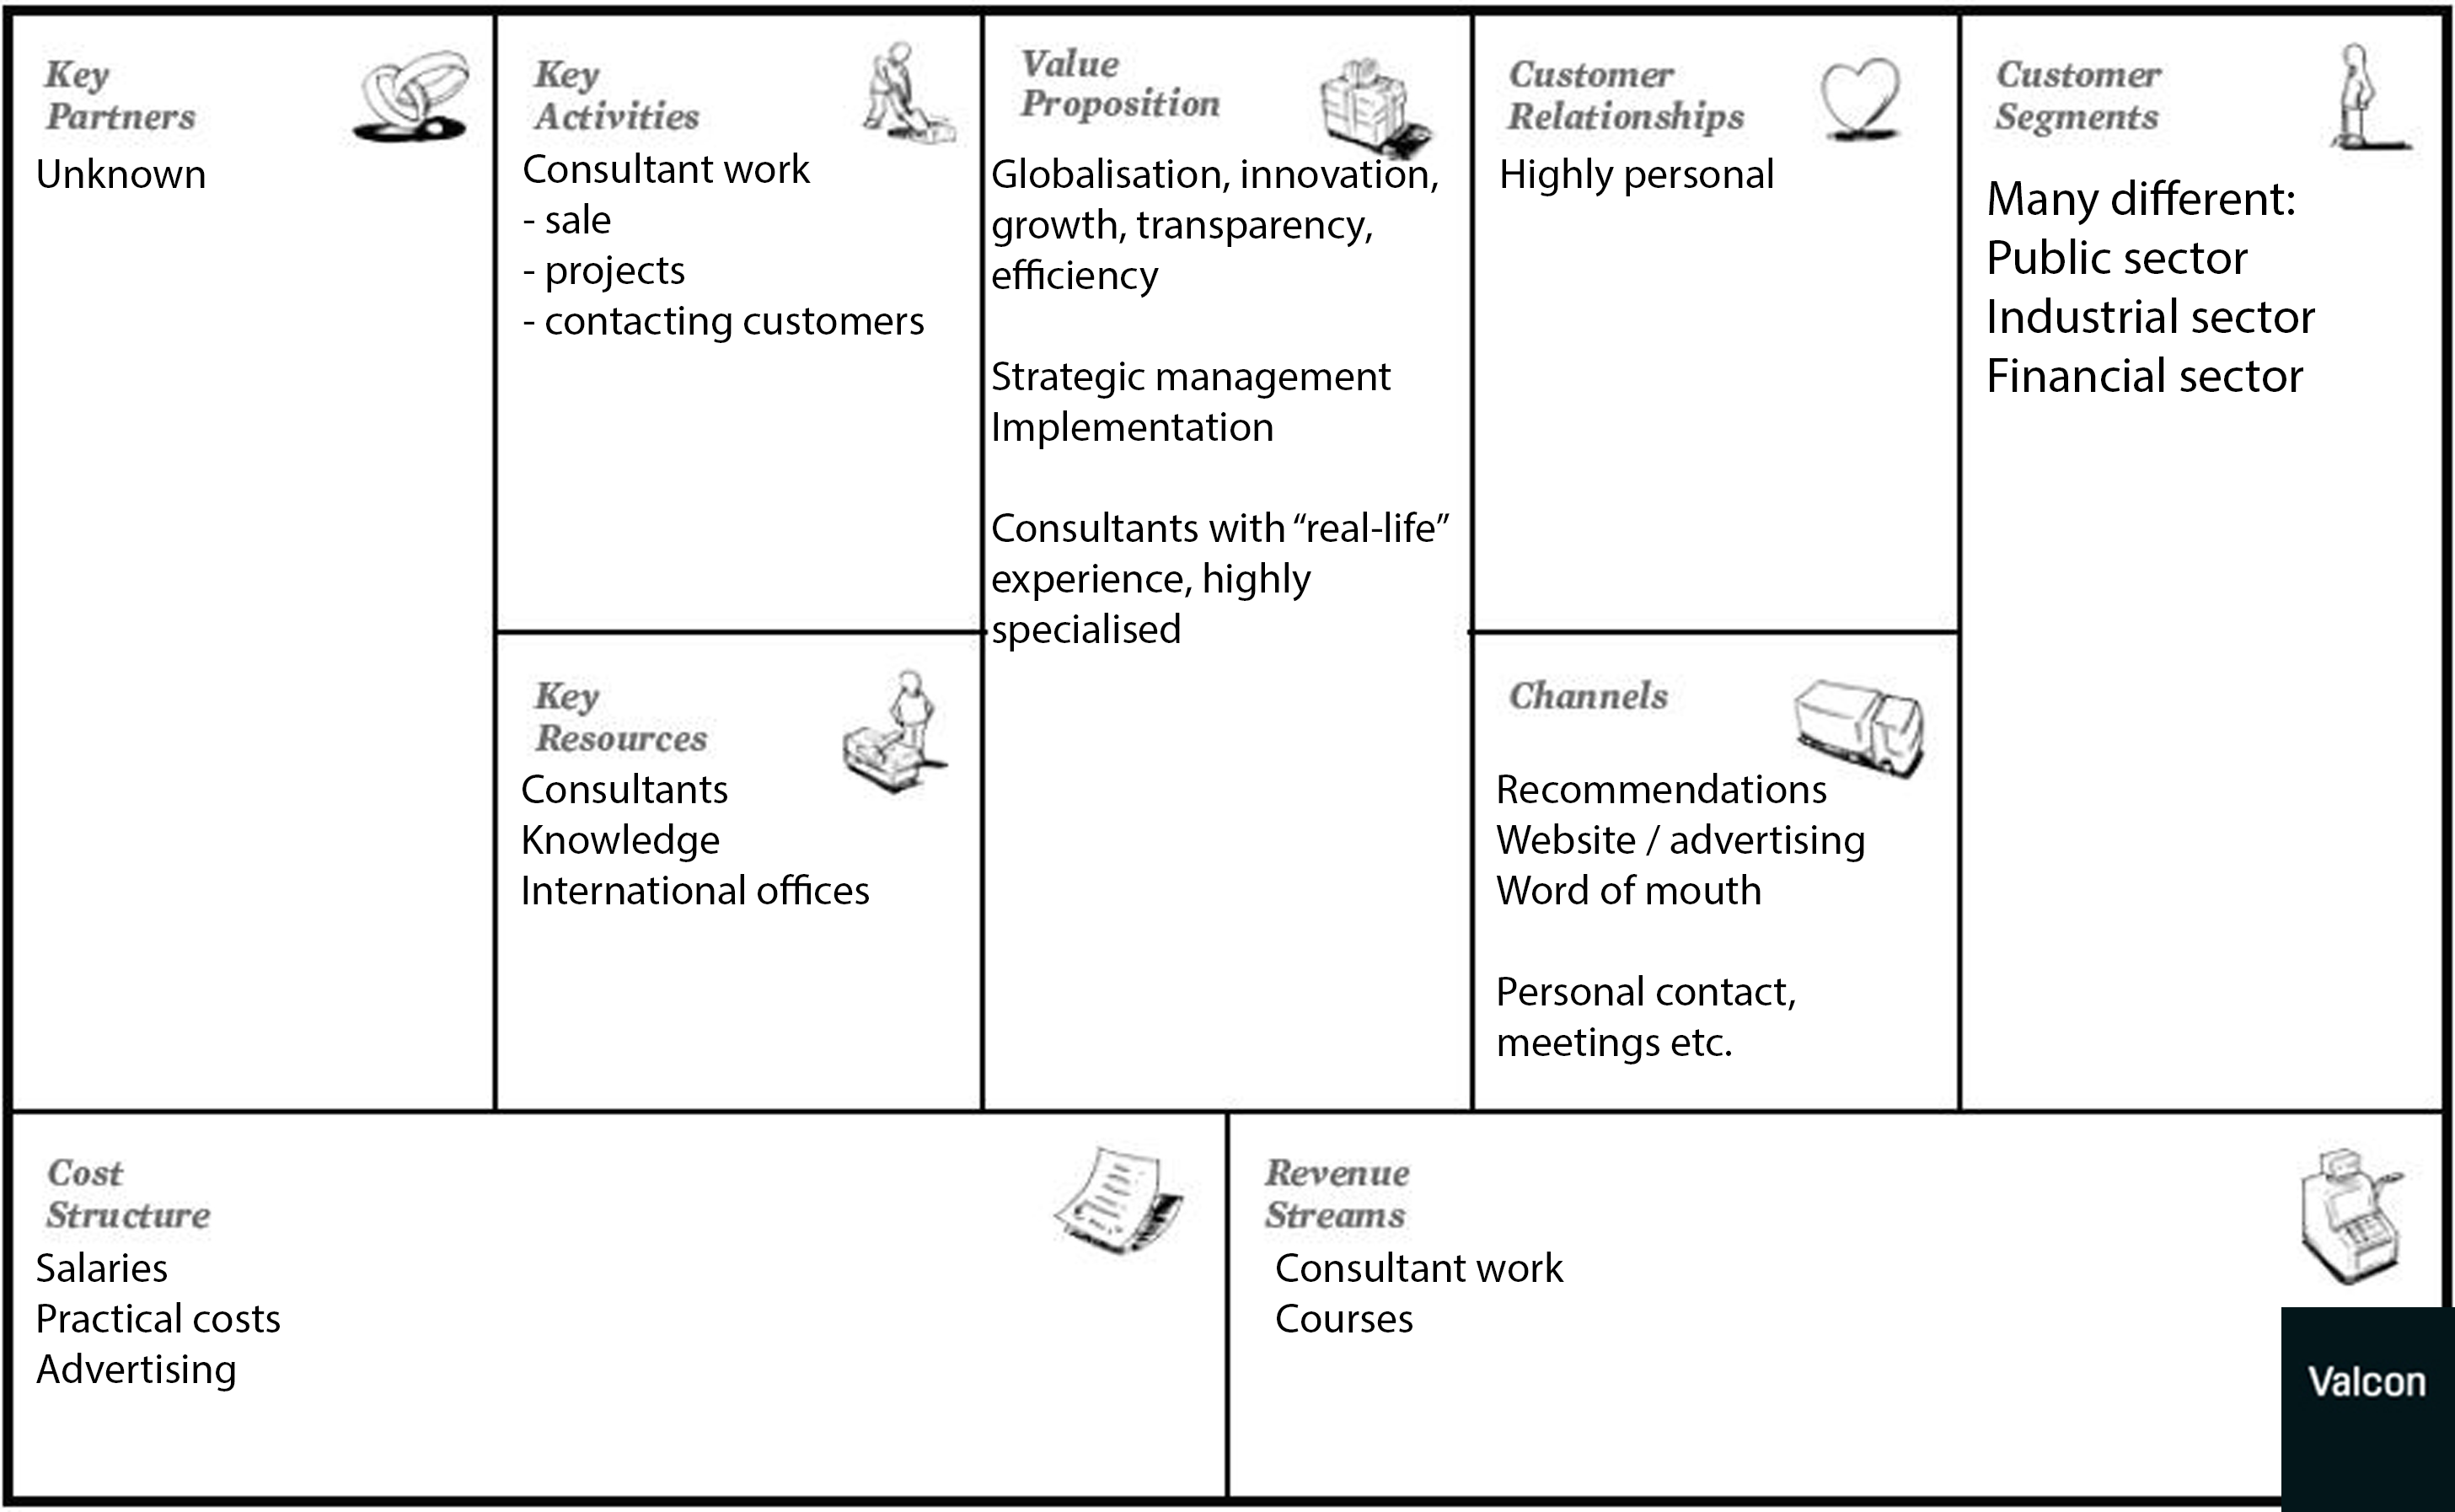
\includegraphics[width=\textwidth]{inline/business-model-canvas.png}
\caption{Valcon's business canvas.}
\label{fig:canvas}
\end{figure}

In relation to the problem it is important to note that the consultants are key resources for Valcon's business
as they are the ones who generate revenue.
As such it is important that they are able to perform their work effectively as soon as they start working at Valcon.
\section{Business strategy, IT strategy and company values}
\subsubsection{Business strategy}
We were not able to acquire Valcon's business strategy, as it is not public and Valcon were not interested in sharing it. (Source: Danni: "Det er korrekt at Valcon gruppens konkrete business strategi ikke er tilgængelig" (appendix \ref{app:business_strategy_refusal})). 
However, we were able to glean some of it through the interviews and meetings:

Valcon is in rapid growth and have a continued focus on keeping this growth as high as possible. 

(Sources: appendix \quoteref{app:danni_initiation}{danni_init_eksplosiv_vekst} and appendix \quoteref{app:danni_initiation}{danni_init_business_strategy_vekst}).

\subsubsection{IT strategy}
Valcon's IT strategy focuses on streamlining IT activities, being cost efficient, outsourcing labor intensive tasks, making work easier for the consultants, few but strong partnerships and choosing off-the-shelf systems instead of customized systems.

See appendix \ref{app:it_strategy} for the original document.

\subsubsection{Company values}
Valcon is guided by four values internally: Integrity, joy, performance, and competence.
Furthermore they value a flat hierarchy.
(Source: appendix \quoteref{app:danni_initiation}{danni_init_firmastruktur}).
\section{Work domains}
Entering newly hired employees into the systems at Valcon and requisitioning the required hardware is currently a stressful process.

Initiators of the process in both Valcon and OMT send information to accounting, who proceeds to enter information into some systems while IT enters information into other systems, sets the hardware for the new employee up, and sends it to him/her.
The new employee is contacted both by the initiators and IT, and sometimes by accounting as well.

But the core of the problem is that the process sometimes has to be very quick.
In that case, the initiators initiate the process both in IT and accounting at the same time, leading to more stress and intercommunication between them.

Looking at the process it seems essential to take a deeper look at the following work areas in order to get a better understanding of the problem:
\begin{itemize}
\item Recruitment (the initiators)
\item Accounting
\item IT
\end{itemize}

A visual representation of the organization as well as the work domains to research can be seen in appendix \ref{app:OrganizationalChart}
\section{Conclusion}
This section aims to explain how the recruitment process problem, we are dealing with, is relevant to Valcon as a whole.\\

\noindent Part of Valcon's business strategy is to keep a high growth rate for the company.
A high growth rate means many new employees.
All employments go through Group Support Functions (IT and accounting) in the recruitment process.
Group Support Functions has problems dealing with the current amount of employments.

Since Valcon intends to keep growing and Group Support Functions have problems keeping up, there is a need to optimize the process.